\documentclass[11pt, oneside]{article}   	% use "amsart" instead of "article" for AMSLaTeX format
\usepackage{geometry}                		% See geometry.pdf to learn the layout options. There are lots.
\usepackage{textcomp}
\usepackage{hyperref}  % TODO: see page 94 of latex book
\geometry{letterpaper}                   		% ... or a4paper or a5paper or ... 
%\usepackage[parfill]{parskip}    		% Activate to begin paragraphs with an empty line rather than an indent
\usepackage{graphicx}				% Use pdf, png, jpg, or eps§ with pdflatex; use eps in DVI mode
								% TeX will automatically convert eps --> pdf in pdflatex		
\usepackage{amssymb}
\usepackage{relsize}

\title{CSCI 181 / E-181 Spring 2014 Practical 2}

\author{
  David Wihl\\
  \texttt{davidwihl@gmail.com}
  \and
  Zack Hendlin\\
  \texttt{zgh@mit.edu}
}
%\date{}							% Activate to display a given date or no date

\begin{document}
\maketitle
\section*{Warm-Up}

%max g-forces eyeballs out is 12g eyeballs out http://www.gforces.net/human-tolerance-horizontal.html

%helmet tests on g forces http://www.smf.org/docs/articles/hic/Various_helmets_stds.pdf

\subsection*{Baseline}

\begin{figure}[h!] 
  \centering
  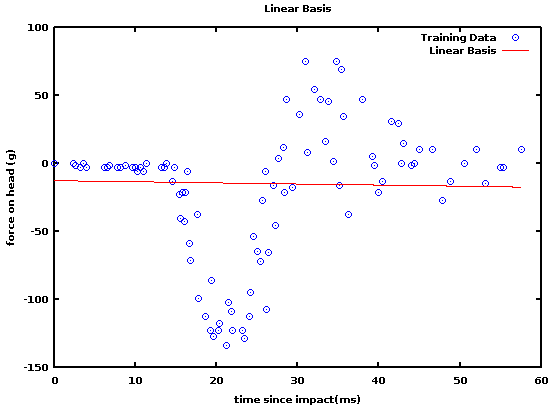
\includegraphics[scale=0.6]{gradient_descent}
  \caption{Warmup: Linear Basis\label{gradientdescent}}
\end{figure}

As a baseline, we first created a simple linear gradient descent with a flat slope and intercept. 

We also used a polynomial basis, iterating with polynomials from $n^2$ up to $n^{12}$ and selecting the lowest error. Unsurprisingly, $n^{12}$ had the lowest error rate, but is likely highly overfit.

\begin{figure}[h!] 
  \centering
  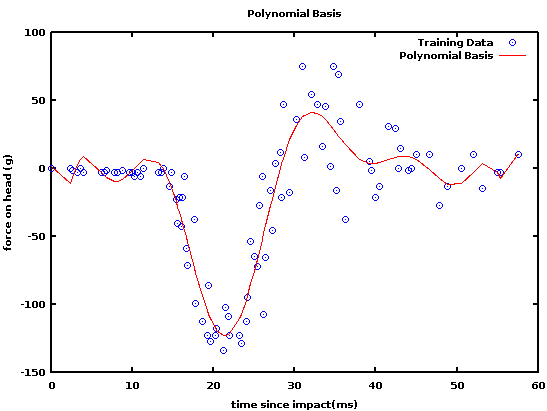
\includegraphics[scale=0.6]{polyfit}
  \caption{Warmup: Polynomial Basis $n^{12}$}
\end{figure}

\subsection*{Bayesian Linear Regression}

Using Gaussian Likelihood and Prior, we solved for $W$ using Moore Penrose.
\begin{equation}
W_{ML} = (\Phi^T\Phi)^{-1}\Phi^Tt
\end{equation}

This was simple to implement, especially in Octave/Matlab. However, without normalization the error rate was close to the baseline linear basis and significantly worse than the polynomial.

\begin{figure}[h!] 
\centering
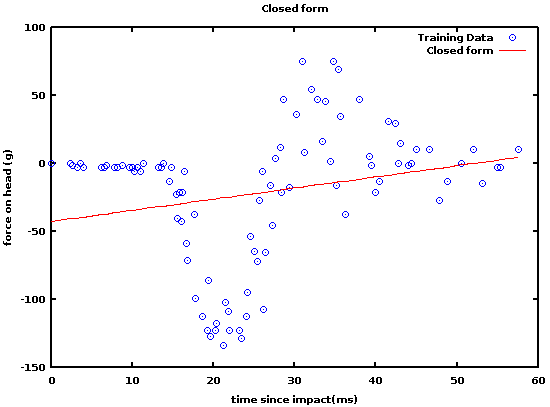
\includegraphics[scale=0.6]{closed_form}
\caption{Warmup: Gaussian}
\end{figure}


\subsection*{Locally Weighted Linear Regression}

Locally Weighted Linear Regression\footnote{\emph{Machine Learning in Action} by Peter Harrington. \textsuperscript{\textcopyright} 2012 ISBN 978-1617290183} provided the lowest cost overall and a smooth fit to the data without overfitting given the profile of this dataset. A variety of $K$ values were attempted. 0.001 never converged. Values from 0.5, 1.0, 5.0 and 10.0 did converge with 1.0 seemingly providing the best balance between fit and smoothness.




\begin{figure}[h!] 
\centering
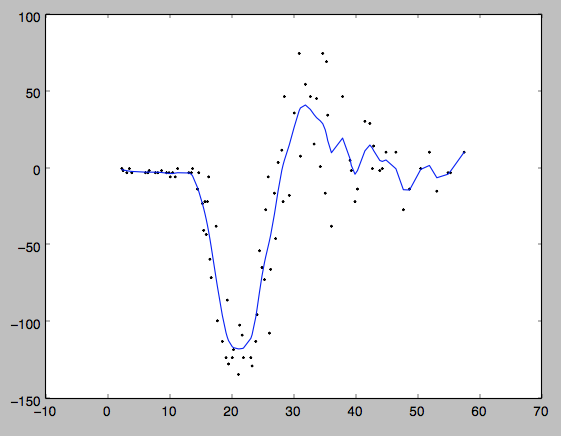
\includegraphics[scale=0.6]{lwlr}
\caption{Warmup: Locally Weighted Linear Regression $K=1$}
\end{figure}

\subsection*{Warmup Summary}

The following table summarizes our results. LWLR was reasonably simple to implement and provided the lowest cost. For this particular data set, it would be our basis function of choice.

\begin{center}
    \begin{tabular}{| l | l |}
    \hline
    Basis & Lowest Error \\ \hline
    Linear Basis & \hfill 1293.0 \\
    Gaussian Basis & \hfill 1187.7 \\
    Polynomial Basis & \hfill 211.9 \\
    LWLR Basis & \hfill 185.6 \\
    \hline
    \end{tabular}
\end{center}


\section*{Predicting Movie Opening Weekend Revenues}


\subsection*{Subsection 1}

\subsection*{Subsection 2}

\section*{Conclusion}


\end{document}  
